% Barrido de fortaleza de los monitores, en pgfplots.
%
% Datos: results/machine-A/corpus/monitor_strength.jsonl, mediana por parametro.
%
% DOS paneles, no uno. Las dos series estan separadas por dos ordenes de
% magnitud, y en un eje compartido el canary queda aplastado contra el cero:
% la figura mostraria la linealidad del heartbeat y escondería la planitud del
% canary, que es la mitad del argumento. Cada panel lleva su escala y el
% lector compara formas, no alturas.
%
% Sin relleno ni color de serie: la distincion la llevan el marcador y el
% trazo, para que siga siendo legible impresa en gris.
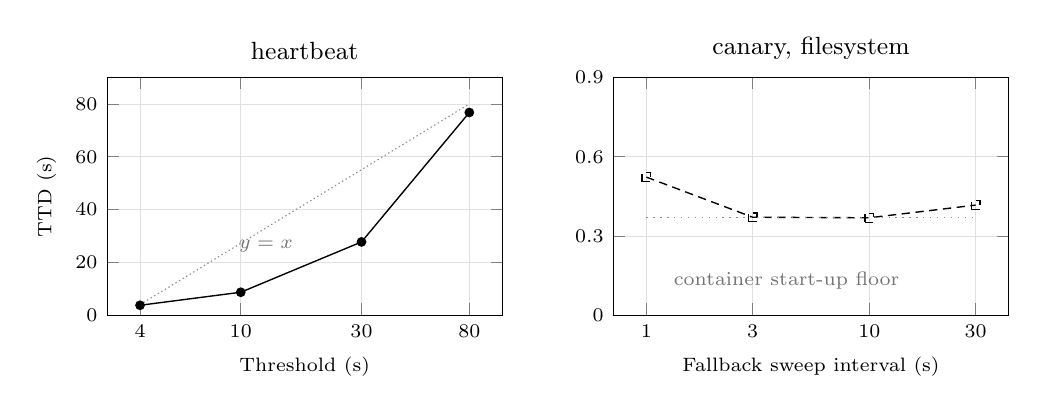
\begin{tikzpicture}

\begin{axis}[
  name=hb,
  width=6.6cm, height=4.6cm,
  xmode=log, log basis x=10,
  xlabel={Threshold (s)}, ylabel={TTD (s)},
  title={\small heartbeat}, title style={yshift=-1mm},
  xtick={4,10,30,80}, xticklabels={4,10,30,80},
  ymin=0, ymax=90, ytick={0,20,40,60,80},
  grid=major, grid style={line width=0.2pt, draw=black!12},
  tick label style={font=\scriptsize}, label style={font=\scriptsize},
  axis line style={line width=0.4pt},
  every axis plot/.append style={line width=0.5pt},
]
\addplot[mark=*, mark size=1.5pt, black] coordinates {
  (4,3.77) (10,8.70) (30,27.76) (80,76.77)
};
% Referencia y=x: si el watchdog fuera perfecto, el TTD igualaria su umbral.
\addplot[densely dotted, black!45, line width=0.4pt, forget plot]
  coordinates {(4,4) (80,80)};
\node[font=\scriptsize, black!55, anchor=west] at (axis cs:9,26) {$y=x$};
\end{axis}

\begin{axis}[
  name=cf, at={(hb.right of south east)}, anchor=left of south west,
  xshift=8mm,
  width=6.6cm, height=4.6cm,
  xmode=log, log basis x=10,
  xlabel={Fallback sweep interval (s)},
  title={\small canary, filesystem}, title style={yshift=-1mm},
  xtick={1,3,10,30}, xticklabels={1,3,10,30},
  ymin=0, ymax=0.9, ytick={0,0.3,0.6,0.9},
  grid=major, grid style={line width=0.2pt, draw=black!12},
  tick label style={font=\scriptsize}, label style={font=\scriptsize},
  axis line style={line width=0.4pt},
  every axis plot/.append style={line width=0.5pt},
]
\addplot[mark=square, mark size=1.6pt, black, densely dashed] coordinates {
  (1,0.523) (3,0.371) (10,0.369) (30,0.417)
};
% El piso real: arrancar el contenedor efimero de prueba, no el monitor.
\addplot[dotted, black!45, line width=0.4pt, forget plot]
  coordinates {(1,0.37) (30,0.37)};
\node[font=\scriptsize, black!55, anchor=south west] at (axis cs:1.2,0.06)
  {container start-up floor};
\end{axis}

\end{tikzpicture}
